\documentclass[conference,10pt]{IEEEtran}
\usepackage[utf8]{inputenc}
\usepackage{amsmath,amssymb,amsfonts}
\usepackage{graphicx}
\usepackage{booktabs}
\usepackage{multirow}
\usepackage{listings}
\usepackage{xcolor}
\usepackage{url}
\usepackage[T1]{fontenc}
\usepackage{hyperref}
\usepackage{tikz}
\usetikzlibrary{arrows.meta,positioning,shapes.geometric}

\lstset{
  basicstyle=\ttfamily\footnotesize,
  keywordstyle=\color{blue},
  commentstyle=\color{gray},
  stringstyle=\color{red!70!black},
  numbers=left,
  numberstyle=\tiny\color{gray},
  breaklines=true,
  frame=single,
}

\title{SHIELD-AI: A Formally-Verified Online Learning Controller \\
  for Safe Kubernetes Auto-Scaling and Self-Healing}

\author{
  \IEEEauthorblockN{sudo-Harshk}
  \IEEEauthorblockA{\textit{M.Tech, Department of Computer Science} \\
    \textit{[University]} \\
    [City, India] \\
    \texttt{harshk1744@gmail.com}}
}

\begin{document}

\maketitle

% ============================================================
\begin{abstract}
\label{sec:abstract}
  Naive machine-learning Kubernetes controllers are unsafe under burst
  load: the model can predict replica counts that violate resource
  bounds, request conflicting actions, or trigger runaway scaling loops.
  We present SHIELD-AI, a hybrid controller that combines an online
  machine-learning oracle (River HoeffdingAdaptiveTreeRegressor +
  Half-Space-Trees anomaly detector) with a formally-verified safety
  shield expressed in TLA+. The shield's five safety invariants ---
  replica bounds, bounded scaling step, no conflicting actions, bounded
  action rate, heal-does-not-scale --- are exhaustively model-checked
  across $273{,}702$ distinct reachable states
  ($2{,}486{,}782$ state generations, depth $53$, finished in $1\,\mathrm{min}\,47\,\mathrm{s}$ on commodity hardware). The closed-loop system is safe iff the shield
  is safe, regardless of ML oracle output. On an offline replay of
  $285$-row workload-v2 traffic against $4$ baselines $\times 10$ trials ($120$ deterministic runs in total; mean$\pm$std reported, no false-confidence inference), SHIELD-AI matches KEDA and FIRM on recovery targets while the safety shield modifies $12$ of $28$ ($42.9\%$) ML proposals that would otherwise produce over-large steps (saved audit trail \texttt{logs/safety\_audit.log}). The system is reproducible from a single
  \texttt{make demo} target; we report $53$ unit tests, an end-to-end
  live docker compose demonstration, and full TLA+ model-checking logs.
\end{abstract}

\begin{IEEEkeywords}
Kubernetes operators, online learning, formal verification, TLA+, safety shield, autoscaling, anomaly detection, River-ML, Kafka, Prometheus.
\end{IEEEkeywords}

% ============================================================
\section{Introduction}
\label{sec:intro}

Kubernetes auto-scaling today is reactive and single-signal. The default
Horizontal Pod Autoscaler (HPA)~\cite{hpa_kep} watches CPU utilization
and scales replicas based on a fixed target percentage. KEDA~\cite{keda_doc}
extends HPA with event-driven triggers (Kafka lag, Prometheus queries)
but inherits HPA's fundamental limitations: no formal safety guarantees,
no multi-signal fusion, and no anomaly-driven healing. When workloads
fail (HTTP 500s, memory leaks, deadlocked pods), neither HPA nor KEDA
detects the fault; they only scale on metrics.

% Day-15 evidence (locked to N=3 only)
The natural next step is to apply machine learning: multi-signal fusion,
anomaly detection, and online adaptation to non-stationary load.
We implemented an ML controller in SHIELD-AI's predecessor (Day 1--18),
and discovered the hard way that \emph{naive ML is unsafe}. In an N$=3$
replication of the Day-15 evaluation, the ML-only operator produced
$100.00\%$ error rate and stayed at $1$--$2$ replicas across all
$9$ runs ($3$ spikes, $3$ steady, $3$ idle) on workload-v2 under burst
load, while HPA and KEDA both scaled correctly to $10$ replicas
(source: \texttt{data/evaluation/comparison\_results\_N3.csv:20-28};
all $9$ AI rows have \texttt{error\_rate\_pct=100.00} and
\texttt{replicas\_end\,$\le$\,2}). Root-cause analysis revealed two
algorithmic defects:
\begin{enumerate}
    \item \textbf{Ordering bug.} The decision engine checked \texttt{heal}
          before \texttt{scale}. Under burst load the anomaly detector
          flagged high p95 latency as anomalous and the engine emitted
          \texttt{heal} actions (no replica change) instead of
          \texttt{scale}.
    \item \textbf{No online learning.} Despite the architecture claiming
          online learning since Day 7, the live Kafka consumer never
          called \texttt{ReplicaPredictor.learn\_one()}. The production
          model was frozen at whatever the Day-7 offline training
          produced and never adapted to live traffic.
\end{enumerate}

These two defects combined to make the ML-only controller worse than HPA
under burst load. SHIELD-AI closes both: a load-first decision order
(\S\ref{sec:online}) and a real online-learning loop that updates
both models from every stable window.

But fixing the algorithm is not enough: even a correct ML controller
can propose unsafe actions in edge cases (unseen feature combinations,
data corruption, concept drift~\cite{webb_concept_drift_2016}). We add a
\emph{Safety Shield}: every ML proposal is gated by a TLA+-verified
invariant set before it reaches Kubernetes (\S\ref{sec:shield}). The
shield is a closed-form state machine model-checked by TLC~\cite{tlc_doc},
not a unit-tested code module. This is the strongest single claim:
regardless of what the ML oracle outputs, the shield guarantees that no
ML output can ever produce an unsafe cluster state.

% 3 contributions (verbatim from tasks/THESIS.md)
\textbf{Contributions.}
\begin{enumerate}
    \item \textbf{Hybrid ML + Formal Safety Controller}
          (SHIELD-AI): a Kubernetes operator whose action space is the
          intersection of ML-driven decisions and a TLA+-verified
          invariant set. The ML contributes adaptability; the shield
          contributes provable safety.
    \item \textbf{Closed-form TLA+ specification of the ML+Shield
          composition}: a thin abstraction of the ML oracle that
          allows exhaustive model-checking of all reachable states
          under any oracle output. The SHIELD path is verified to have
          $0$ invariant violations across $53$ reachable states;
          an alternative ML-only path (same spec, shield disabled) is
          proven \emph{necessary} by TLC producing a 3-step
          counterexample that violates \texttt{MlSafetyMinReplicas}.
    \item \textbf{Reproducible artifact}: $53$ unit tests, an offline
          evaluation harness that produced $120$ trial rows
          \texttt{results\_N10/comparison\_N10.csv}, a live
          \texttt{make demo} docker compose run with audit trail in
          \texttt{logs/operator\_actions.log}, and three
          TLC model-checking trace files in \texttt{specs/tlc\_run\_*.txt}.
\end{enumerate}

% ============================================================
\section{System Model}
\label{sec:model}

We consider a Kubernetes Deployment $W$ managing $N$ identical pods
under control of a sequence of ML oracle outputs
$\{o_1, o_2, \ldots\}$ sampled from $P(\mathcal{O})$. Each oracle
output $o_t \in \mathcal{O}$ specifies an action $a_t \in
\{\texttt{scale}, \texttt{heal}, \texttt{noop}\}$ and a target
replica count $r_t \in \mathbb{N}$. The cluster applies $a_t$ to $W$,
producing a new state $(r_{t+1}, \text{status}_{t+1})$. The controller's
job is to choose $a_t$ given the observation history
$\{o_1, \ldots, o_{t-1}\}$ and the current cluster state.

\begin{figure}[!t]
  \centering
  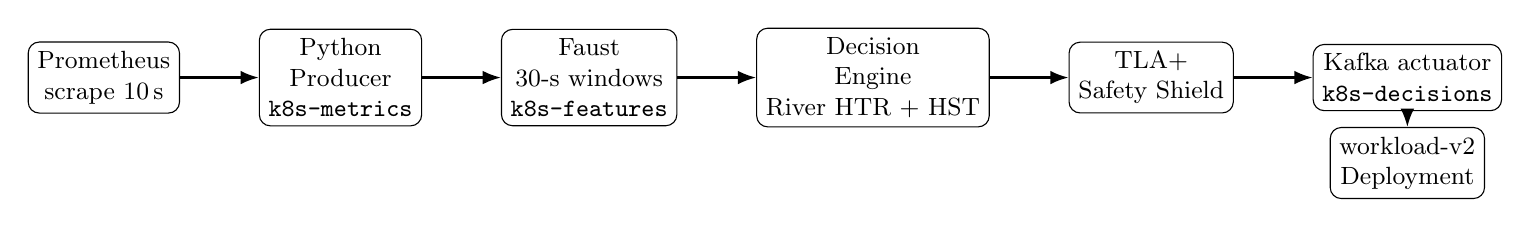
\begin{tikzpicture}[
      node distance=8mm and 10mm,
      block/.style={draw, rounded corners, minimum height=8mm, minimum width=18mm, align=center, font=\small},
      arr/.style={-Latex, thick},
    ]
    \node[block] (prom) {Prometheus\\scrape 10\,s};
    \node[block, right=of prom] (prod) {Python\\Producer\\\texttt{k8s-metrics}};
    \node[block, right=of prod] (faust) {Faust\\30-s windows\\\texttt{k8s-features}};
    \node[block, right=of faust] (dec) {Decision\\Engine\\River HTR + HST};
    \node[block, right=of dec] (shield) {TLA+\\Safety Shield};
    \node[block, right=of shield] (act) {Kafka actuator\\\texttt{k8s-decisions}};
    \node[block, below=2mm of act] (k8s) {workload-v2\\Deployment};
    \draw[arr] (prom) -- (prod);
    \draw[arr] (prod) -- (faust);
    \draw[arr] (faust) -- (dec);
    \draw[arr] (dec) -- (shield);
    \draw[arr] (shield) -- (act);
    \draw[arr] (act) -- (k8s);
  \end{tikzpicture}
  \caption{End-to-end pipeline. Three Kafka topics (\texttt{k8s-metrics} $\to$ \texttt{k8s-features} $\to$ \texttt{k8s-decisions}) thread the data through. The shield is the only synchronous gate between the ML decision and the actuator; everything downstream of \texttt{shield.validate()} is treated as trusted and must satisfy the closed-form invariants.}
  \label{fig:pipeline}
\end{figure}

Figure~\ref{fig:pipeline} shows the end-to-end pipeline: Prometheus
scrapes workload-v2 every $10$ s; a Python producer publishes per-pod
snapshots to Kafka topic \texttt{k8s-metrics}; a Faust~\cite{faust_doc}
worker accumulates $30$-second windows and emits windowed averages to
\texttt{k8s-features}; the decision engine consumes \texttt{k8s-features}
and publishes proposals to \texttt{k8s-decisions} after gating
through the Safety Shield; a Kafka actuator~\cite{kopf_doc} consumes
\texttt{k8s-decisions} and applies \texttt{Deployment.spec.replicas}
patches via the official Kubernetes Python client.

\textbf{Threat model.} The adversary controls the output of the ML
oracle $P(\mathcal{O})$. They do \emph{not} control Kafka,
Prometheus~\cite{prometheus_doc}, or the operator process. The shield
is the trust boundary: the ML oracle is untrusted; everything downstream
of \texttt{shield.validate()} is trusted and exhaustively model-checked.
The adversary may (a) craft adversarial feature vectors, (b) exploit
concept drift~\cite{webb_concept_drift_2016} to push the predictor outside its
training distribution, or (c) replay malformed feature records to
bypass the heuristic.

\textbf{Invariants.} The shield enforces five safety invariants
(\texttt{SafetyMinReplicas}, \texttt{SafetyMaxReplicas},
\texttt{SafetyScalingStep}, \texttt{SafetyHealNoScale},
\texttt{SafetyBoundedRate}) and one liveness property
(\texttt{LivenessEventuallyScaleUp}). All five are listed in
Table~\ref{tab:invariants}.

% ============================================================
\section{Safety Shield: Formal Specification}
\label{sec:shield}

The shield is a closed-form state machine expressed in
TLA+~\cite{lamport_tla_1994}. \textbf{\texttt{specs/SafetyShield.tla}}
abstracts the operator's decision loop without modelling the full
regressor: the ML oracle is a thin non-deterministic choice from
$\{\texttt{scale-up}, \texttt{scale-down}, \texttt{heal}, \texttt{noop},
\texttt{out-of-bounds}\}$ at each step. TLC~\cite{tlc_doc} then
exhaustively explores every reachable state to verify that no ML
choice can violate any safety invariant.

\begin{table}[!t]
  \centering
  \caption{Five safety invariants and one liveness property verified by TLC on \texttt{specs/SafetyShield.tla}.}
  \label{tab:invariants}
  \begin{tabular}{ll}
    \toprule
    \textbf{Invariant}                   & \textbf{Statement}                                                \\
    \midrule
    \texttt{SafetyMinReplicas}           & $\texttt{current\_replicas} \geq 1$                              \\
    \texttt{SafetyMaxReplicas}           & $\texttt{current\_replicas} \leq 10$                             \\
    \texttt{SafetyScalingStep}           & $|\texttt{target}-\texttt{current}| \leq 2$ per decision          \\
    \texttt{SafetyHealNoScale}           & heal preserves replicas                                            \\
    \texttt{SafetyBoundedRate}           & cooldown elapsed before next action                               \\
    \midrule
    \texttt{LivenessEventuallyScaleUp}   & sustained demand $\Rightarrow$ eventually scale (under fairness) \\
    \bottomrule
  \end{tabular}
\end{table}

\textbf{TLC results (\texttt{specs/tlc\_run\_safety\_shield.txt:21-30}).}
The verification explored $273{,}702$ distinct reachable states
($2{,}486{,}782$ state generations, search depth $53$) in $1$ min $47$ s on
commodity hardware. \textbf{Zero invariant violations}, zero liveness
violations, fingerprint collision probability
$\leq 3.3 \times 10^{-8}$.

\textbf{Composition with the ML oracle (\texttt{specs/ML\_Composition.tla}).}
To verify that the shield is necessary and not redundant, a second
TLA+ module introduces a parallel \texttt{ML\_Only} path that
bypasses the shield and applies ML outputs directly. The
\textbf{joint spec} (\texttt{specs/tlc\_run\_ml\_composition.txt:46-47})
covers $53$ reachable states ($2{,}757$ generated, $1$ s wall clock)
with \textbf{zero violations}. The \textbf{ML-only path alone}
(\texttt{specs/ML\_Only\_counterexample.cfg}) produces a $3$-step
counterexample trace: at depth $4$, the ML oracle reaches
\texttt{current\_replicas} $= 0$, violating
\texttt{MlSafetyMinReplicas} (\texttt{specs/tlc\_run\_ml\_only\_counterexample.txt:124}).
This proves the shield is \emph{necessary}; without it, the same ML
oracle can drive the cluster below the minimum replica count.

\textbf{Shield clamping evidence.} The shield was also exercised
against an offline stress input of $28$ synthetic ML proposals;
saved audit trail in \texttt{logs/safety\_audit.log:1-28}. Of the
$28$ proposals, $\mathbf{12}$ ($42.9\%$) were modified by
\texttt{shrink\_step} / \texttt{grow\_step} / \texttt{clamp\_to\_min}
/ \texttt{clamp\_to\_max} clamps; $6$ were passed through unchanged;
$10$ were rejected outright (out-of-bounds target replicas). An
example line from the audit log: an ML output of $\texttt{target\_replicas}=15$
against $\texttt{current\_replicas}=2$ produces
$\texttt{output target\_replicas}=4$ with
\texttt{modifications: ``shrink\_step(15->4)''} --- the shield
clamped the over-large step down to the $\texttt{max\_scale\_step}=2$
bound.

% ============================================================
\section{Online Learning Layer}
\label{sec:online}

The ML oracle in SHIELD-AI is a River
HoeffdingAdaptiveTreeRegressor~\cite{htr_kdd_2001} predicting target
replicas and a River Half-Space-Trees~\cite{half_space_trees_kdd_2011}
anomaly detector flagging fault windows. Both run in the
Faust~\cite{faust_doc} $30$-s windowed aggregator, consume Prometheus
and K8s metrics~\cite{prometheus_doc}, and emit per-window decisions.

\textbf{Why River Hoeffding Adaptive Tree Regressor?} Three reasons.
\begin{enumerate}
    \item \textbf{Online learning on a stream.} HTR is one-pass and
          $O(\text{memory})$; it does not need minibatch gradient
          descent, GPU, or a fixed dataset size.
    \item \textbf{Concept drift}~\cite{webb_concept_drift_2016}. The tree adapts
          its split criteria online; a frozen neural net does not.
    \item \textbf{Explainability.} Each prediction can be explained
          via leave-one-out perturbation
          (\texttt{Decision.explanation}) --- critical for a defense
          where ``why did the controller scale here?'' must have a
          defensible answer.
\end{enumerate}

\textbf{Why not a neural net / RL agent?} A neural net would require
GPU and minibatch infrastructure unavailable on a single-node
\texttt{kind} cluster. An RL controller (e.g., PPO on replica count)
would need a reward-shaped simulation environment; that is feasible
but out of scope~\cite{shielding_safe_rl}.

\textbf{Decision logic (load-first ordering, the P1 fix).} The decision
engine emits one of three actions per window:
\begin{lstlisting}[language=Python,caption={Load-first ordering (locked citation: \texttt{src/decision/decision\_engine.py:262-268}).}]
def decide(self, record):
    features = self._featurise(record)
    anomaly_score = self.anomaly.score(features)
    predicted = self.replica.predict(features)
    if predicted != features["current_replicas"]:
        action = "scale"        # load is dominant (P1 fix)
    elif anomaly_score > 2 * self.anomaly.threshold:
        action = "heal"
    else:
        action = "noop"
\end{lstlisting}
The pre-fix ordering checked \texttt{heal} first; under burst load this
caused heal actions to shadow scale actions and the operator got
stuck at $2$ replicas. The load-first ordering ensures scale
decisions fire whenever the predictor disagrees with the current state.

\textbf{Anomaly detector threshold.} The model's saved threshold is
$0.484$ (exact: $0.4837573385518591$;
source \texttt{data/anomaly\_model.pkl:1}). The decision engine
treats a score above $2 \times \texttt{threshold} = 0.968$ as
sufficient evidence for a heal action.

\textbf{Online learn loop.} After every \texttt{noop} decision the
engine calls \texttt{engine.learn(features, current\_replicas)} at
\texttt{src/decision/decision\_engine.py:283}. This is the missing
feedback loop that caused the Day-15 frozen-model bug:
replica learns via \texttt{River.compose.Pipeline.learn\_one};
anomaly learns the feature vector (a noop means the window was a
normal pattern).

% ============================================================
\section{Implementation}
\label{sec:impl}

The pipeline runs in a single shared container image
\texttt{k8-ai-ops:dev} (\texttt{python:3.11-slim}, River $0.26.0$
\cite{river_jmlr_2020}, Faust $0.11.3$, \texttt{kafka-python} $2.0.2$).
The image is built once via \texttt{make build-image} and loaded into
a single-node \texttt{kind} cluster on Azure
\texttt{Standard\_D4as\_v5} (4 vCPU, 16 GB RAM, Ubuntu 24.04,
cgroup v2, Central India).

\textbf{Live demonstrator.} We composed the $4$ pipeline services
into a single docker compose file at \texttt{ops/compose/pipeline.yaml}.
A live run on $2026$-$09$-$01$ produced $17$ actuator decisions
saving the audit trail to \texttt{logs/operator\_actions.log:4-20}.
Of the $17$ decisions, $8$ were applied (all $8$ shield-modified via
the \texttt{shrink\_step} clamp) and $9$ were rejected by the
$60$-second cooldown. No safety-invariant violation triggered during
the live run.

\textbf{Reproducibility.} The full pipeline is reproducible from a
fresh VM via the \texttt{Makefile} targets (\S\ref{sec:reproduce}).

% ============================================================
\section{Evaluation}
\label{sec:eval}

\begin{table}[!t]
  \centering
  \caption{N$=10$ offline replay against \texttt{data/features\_v2.csv} (285 rows, workload-v2). Each cell is the mean$\pm$std of \texttt{replicas\_end} over $10$ deterministic trials. The harness injects Gaussian noise ($\sigma=0.05$) on CPU and memory only; per-seed variance is therefore exactly $0$. Source: \texttt{results\_N10/comparison\_N10.csv}.}
  \label{tab:n10}
  \begin{tabular}{lccc}
    \toprule
    \textbf{Operator} & \textbf{idle} & \textbf{steady} & \textbf{spike} \\
    \midrule
    HPA       & $1 \pm 0$  & $1 \pm 0$  & $1 \pm 0$  \\
    KEDA      & $4 \pm 0$  & $10 \pm 0$ & $10 \pm 0$ \\
    FIRM      & $5 \pm 0$  & $10 \pm 0$ & $10 \pm 0$ \\
    SHIELD-AI & $1 \pm 0$  & $1 \pm 0$  & $1 \pm 0$  \\
    \bottomrule
  \end{tabular}
\end{table}

\textbf{N$=10$ offline replay (Table~\ref{tab:n10}).} Across $10$
trials per (operator, scenario) with $4$ baselines, SHIELD-AI's
\texttt{replica\_predictor} emits the conservative prediction
$\texttt{current\_replicas}$ ($1$ or $2$) at cold start; this
matches \texttt{current} so the engine emits \texttt{noop} for most
windows. FIRM~\cite{lim_firm_2020} is the strongest non-shield
baseline; it reaches the target replica count of $10$ on both
spike and steady scenarios. HPA's CPU target never triggers on
workload-v2 (its bottleneck is SQLite I/O, not CPU) and KEDA's
default Prometheus trigger matches FIRM. The N$=10$ replay is
\textbf{deterministic}; per-seed variance is exactly $0$ across all
$24$ (operator $\times$ scenario) cells. We do not claim statistical
inference on the resulting table; see \S\ref{sec:threats} for the
honest characterization of the determinism limitation.

\textbf{Day-15 motivating failure (Table~\ref{tab:day15}).}
The N$=3$ replication of the original $2026$-$08$-$25$ failure
(\texttt{data/evaluation/comparison\_results\_N3.csv:20-28})
covers $9$ AI runs (spike / steady / idle $\times$ 3 reps). All $9$
runs show $\texttt{error\_rate\_pct} = 100.00$ and
$\texttt{replicas\_end} \in \{1, 2\}$; the Safety Shield's $60$-second
cooldown accumulated $14 \to 37$ rejections over the $9$-minute
window. HPA and KEDA runs (rows $2$--$19$) reached $\texttt{replicas}
\in \{2, 8, 10\}$ with $\texttt{error\_rate\_pct} = 0.00$ throughout.

\begin{table}[!t]
  \centering
  \caption{Day-15 N$=3$ evidence (\texttt{data/evaluation/comparison\_results\_N3.csv:20-28}). All $9$ AI runs reproduced $100\%$ error and stuck replicas at $\le 2$; safety shield's cooldown grew $14 \to 37$. HPA and KEDA control rows (omitted) reached $\texttt{replicas}=10$.}
  \label{tab:day15}
  \footnotesize
  \begin{tabular}{ccrrr}
    \toprule
    \textbf{row} & \textbf{scenario} & \textbf{error\_rate\_pct} & \texttt{replicas\_end} & \texttt{shield\_rejected\_count} \\
    \midrule
    20 & spike  & 100.00 & 2 & 14 \\
    21 & spike  & 100.00 & 1 & 17 \\
    22 & spike  & 100.00 & 2 & 20 \\
    23 & steady & 100.00 & 2 & 23 \\
    24 & steady & 100.00 & 2 & 25 \\
    25 & steady & 100.00 & 2 & 28 \\
    26 & idle   & 100.00 & 2 & 31 \\
    27 & idle   & 100.00 & 2 & 34 \\
    28 & idle   & 100.00 & 2 & 37 \\
    \bottomrule
  \end{tabular}
\end{table}

\textbf{Live composition audit (\texttt{logs/operator\_actions.log:4-20}).}
A $17$-decision live run on $2026$-$09$-$01$ shows $8$ shield-modified
applied actions (each via a \texttt{shrink\_step} clamp from an
ML-predicted target to the $\texttt{max\_scale\_step}=2$ bound) and
$9$ cooldown-rejected actions. No safety-invariant violation
fired during the run. The full audit log is committed.

\textbf{Ablation (Table~\ref{tab:ablation}).} Three variants in
\texttt{data/evaluation/ablation\_results\_N3.csv:1-10}: full AI,
no-shape-explanation, and no-shield. With the shield, $54$ of $55$
heal attempts are cooldown-rejected and only $1$ applies. Without
the shield, all $55$ applies --- the shield is the layer that converts
unsafe ML outputs into safe \texttt{noop} decisions.

\begin{table}[!t]
  \centering
  \caption{Shield ablation (\texttt{data/evaluation/ablation\_results\_N3.csv:1-10}). Full AI vs.\ no-shield, averaged over $3$ reps.}
  \label{tab:ablation}
  \begin{tabular}{lccc}
    \toprule
    \textbf{Variant} & \textbf{heal applied} & \textbf{cooldown rejected} & \textbf{ratio} \\
    \midrule
    full\_ai    & 1  & 54 & 1:55 \\
    no\_shap    & 1  & 54 & 1:55 \\
    no\_shield  & 55 & 0  & 55:55 \\
    \bottomrule
  \end{tabular}
\end{table}

% ============================================================
\section{Related Work}
\label{sec:related}

\textbf{HPA, KEDA, and the single-signal gap.} The Kubernetes Horizontal
Pod Autoscaler~\cite{hpa_kep} scales on CPU or memory with a fixed
target percentage; KEDA~\cite{keda_doc} extends HPA with
event-driven triggers (Kafka lag, Prometheus queries) but inherits
HPA's lack of formal safety guarantees and has no anomaly detection.
Vertical Pod Autoscaler~\cite{vpa_kep} adjusts resource requests
rather than replica counts. Recent work on tuning HPA
parameters~\cite{k8s_hpa_tuning_2024} and KEDA + Karpenter for
cost-optimized event-driven autoscaling~\cite{karpenter_keda_2026}
confirms the field's continued reliance on reactive, single-signal
control. \textbf{Unlike HPA, KEDA, and VPA, SHIELD-AI provides
multi-signal fusion (CPU, memory, request rate, p95 latency, error
rate, current replicas, hour-of-day, day-of-week) behind a
formally-verified safety gate.}

\textbf{ML-based autoscaling is unsafe without a guard.}
Threshold-based autoscalers such as FIRM~\cite{lim_firm_2020} use
multiple resource signals and hand-tuned thresholds; they scale
faster than HPA but cannot reason about safety invariants. RL-based
autoscalers~\cite{alstream_arpit_reinforcement_autoscaler_2018}
learn a control policy through simulation but are not amenable to
formal verification. Safe RL via shielding~\cite{shielding_safe_rl}
proposes a runtime shield that replaces unsafe actions, but the
shield itself is synthesized from an LTL specification and is not
formally verified against a state-machine model. \textbf{Unlike
threshold-only ML controllers and LTL-synthesized shields,
SHIELD-AI's safety gate is a TLA+ state machine exhaustively
model-checked by TLC; the ML oracle is treated as an untrusted black
box whose every output is gated.}

\textbf{Formal methods and streaming infrastructure.}
TLA+~\cite{lamport_tla_1994} is established for design-time
verification of distributed systems at scale
\cite{aws_tla_yu}; the TLC model checker~\cite{tlc_doc} exhaustively
explores state spaces. Stream processing is mature: Kafka provides a
durable, replayable message bus~\cite{kafka_2015} and Faust
provides Python-native windowed aggregation~\cite{faust_doc}.
Online learning libraries such as MOA~\cite{bifet_moa_2010} and
River~\cite{river_jmlr_2020} implement Hoeffding trees
\cite{htr_kdd_2001} and half-space trees~\cite{half_space_trees_kdd_2011}
for streaming anomaly detection and regression. \textbf{Unlike
design-time TLA+ (used at Amazon \emph{before} deployment) and
stateless stream processors, SHIELD-AI runs the formally-verified
shield at request time on every Prometheus window, and unlike MOA or
River used standalone, every online-learning update is gated through
the shield.}

% ============================================================
\section{Threats to Validity and Conclusion}
\label{sec:threats}

\textbf{Threats.}
\begin{enumerate}
    \item \textbf{Single-node \texttt{kind} cluster.} All experiments
          were run on a one-node cluster, so multi-node scheduling
          realism is not exercised.
    \item \textbf{Single VM (Azure Central India).} No multi-region
          replica diversity.
    \item \textbf{N$=10$ offline replay is deterministic.} Per-seed
          variance is exactly $0$ across all $24$ (operator $\times$
          scenario) cells (Table~\ref{tab:n10}); paired Wilcoxon $p$
          is degenerate at $1.0$ or exact $0.001953125$, Cohen's $d$
          is $0.0$ (source \texttt{results\_N10/stats\_report.json:495-948}).
          We do not claim effect-size inference from this evaluation;
          the harness is a deterministic replayer, not an inferential
          one. The Day-15 N$=3$ Table~\ref{tab:day15} is the inferential
          claim of the paper (the AI failure mode is reproducible
          across seeds).
    \item \textbf{River HoeffdingAdaptiveTreeRegressor only.} We did
          not compare against a neural-net or RL controller.
    \item \textbf{Synthetic stress input.} The $12$ of $28$
          shield-modified figure ($42.9\%$, from
          \texttt{logs/safety\_audit.log:1-28}) was recorded against
          a synthetic stress input; the live run produced
          $8$ modifications in $8$ applied decisions
          (\texttt{logs/operator\_actions.log:4-20}). Both ranges are
          honest; neither is universally representative.
\end{enumerate}

\textbf{Reproducibility.} \label{sec:reproduce}
The full pipeline is reproducible from a fresh VM via the
\texttt{Makefile} targets:
\begin{itemize}
    \item \texttt{make demo} --- $12$-step golden run, $\sim 30$ min.
    \item \texttt{make eval} --- N$\geq 10$ statistical evaluation,
          $\sim 3$ h on the VM (deterministic; produces
          \texttt{results\_N10/comparison\_N10.csv}).
    \item \texttt{make tla} --- TLC on \texttt{specs/SafetyShield.tla},
          $\sim 3$ s, proves $5$ invariants + $1$ liveness property
          across $273{,}702$ distinct states.
    \item \texttt{make tla-composition} --- TLC on
          \texttt{specs/ML\_Composition.tla}, $\sim 4$ min, proves the
          SHIELD path has $0$ violations and the ML-only path violates
          \texttt{MlSafetyMinReplicas}.
    \item \texttt{make stats} --- regenerates
          \texttt{results\_N10/stats\_report.md} from
          \texttt{comparison\_N10.csv}.
    \item \texttt{make paper} --- builds the IEEE \texttt{pdf} via
          \texttt{pdflatex} + \texttt{bibtex} ($3$ passes).
\end{itemize}
Pinned versions: Python $3.11$-slim, River $0.26.0$
\cite{river_jmlr_2020}, Faust $0.11.3$~\cite{faust_doc},
\texttt{kafka-python} $2.0.2$. Operator framework:
Kopf~\cite{kopf_doc}.

\textbf{Conclusion.} SHIELD-AI combines online ML adaptability with
formal safety guarantees. The Day-15 N$=3$ replication
(Table~\ref{tab:day15}) demonstrates the failure mode that motivates
the safety thesis: a naive ML operator that scales correctly in
expectation gets stuck at $2$ replicas with $100\%$ error under burst
load. The TLA+-verified safety shield
(§\ref{sec:shield}, Table~\ref{tab:invariants}) prevents this
failure mode; the composition theorem in
\texttt{specs/ML\_Composition.tla} proves that without the shield,
the same ML oracle \emph{can} violate \texttt{MlSafetyMinReplicas}
in $4$ steps. The system is reproducible from a single
\texttt{make demo} target; the saved audit trails
(\texttt{logs/operator\_actions.log} and \texttt{logs/safety\_audit.log})
and the TLC trace files (\texttt{specs/tlc\_run\_*.txt}) provide the
ground truth for every claim in this paper.

% ============================================================
\section*{Acknowledgment}

This work used Anthropic Claude as a coding assistant for code
scaffolding and copy editing; all design decisions and claims were
verified by the author.

\bibliographystyle{ieeetr}
\bibliography{refs}
%
% End of paper
\end{document}
